\section{Background}
\label{sec:background}

In this section, we provide a background on the state-of-the-art RDAs (\Cref{ssec:rda}) that \name{} targets by reading and transforming an Input Graph (\Cref{ssec:igraph}) generated from a high-level programming language.

\subsection{Reconfigurable Dataflow Accelerator (RDA)} 
\label{ssec:rda}

RDAs are high-throughput, low-latency, and energy-efficient architecture providing flexible datapath
and streaming dataflow execution.
RDAs are designed as (multi-level) hierarchical architectures to provide better resource density in a scalable fashion. 
The hierarchical network allows RDA to maintain a fixed high clock frequency at a large scale in contrast to an FPGA.
\Cref{fig:arch} depicts an RDA with two-levels of hierarchy.
At the outer-level, an RDA is configured as a pool of distributed physical blocks (PBs) that are interconnected via a global network (an ultra high-bandwidth all-to-all streaming network).
Whereas, at the inner-level, each PB consists of compute and memory elements connected through a reconfigurable data path.
Communication latency within PBs, between local compute and memory resources, is a single cycle (guaranteed); 
while access across PBs can take variable and potentially unpredictable amounts of latency due to DRAM access or dynamic network congestion.

Inside PBs, the compute can be implemented using a systolic array~\cite{DaDianNao}, DySER array~\cite{dyser}, FPGA fabric, or SIMD pipeline~\cite{plasticine}.
The on-chip memory is often in the form of an SRAM or an eDRAM, behaving as an explicitly managed scratchpad.
Unlike CPUs with cache-coherent memories, in RDAs, a software manages transfers between scratchpads and off-chip memories---mitigating the substantial performance and energy 
overhead due to cache coherency~\cite{mark}.
Other resources, within PBs, are input buffers (for streaming data from the network) and configurable counter (to keep track of local state).
Furthermore, PBs can differ in the type and amount of resources they hold. 
For instance, there can be specialized PBs for generating DRAM requests that are less arithmetic-intensive than regular PBs.

\begin{figure}[!tbp]
\centering
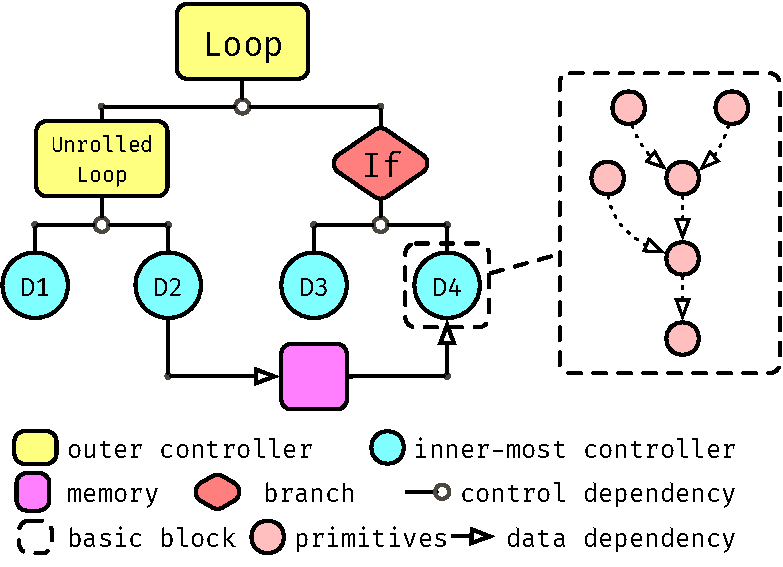
\includegraphics[height=0.13\paperheight]{figures/controller_ir.pdf}
\caption{Input Control- and Data-Flow Graph for \name{}}
\label{fig:controller}
\centering
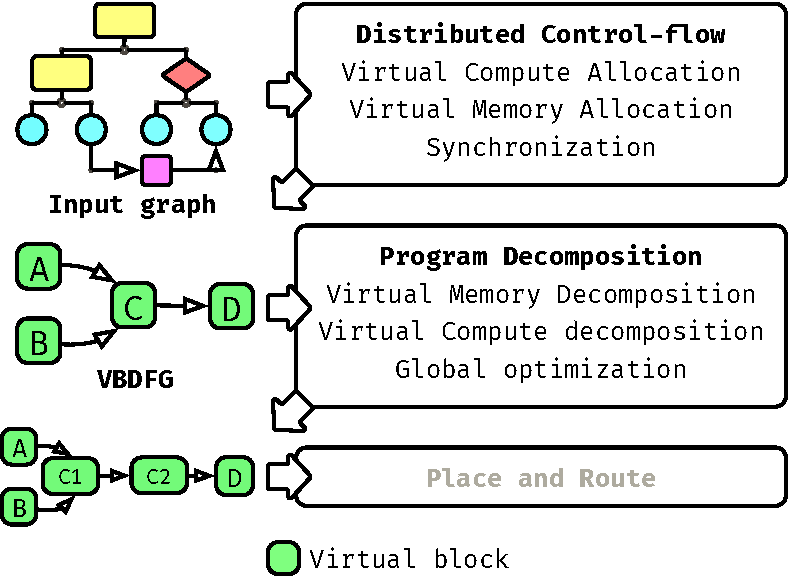
\includegraphics[width=0.8\columnwidth]{figures/compiler_pass.pdf}
\caption{Compilation Phases.}
\label{fig:flow}
\centering
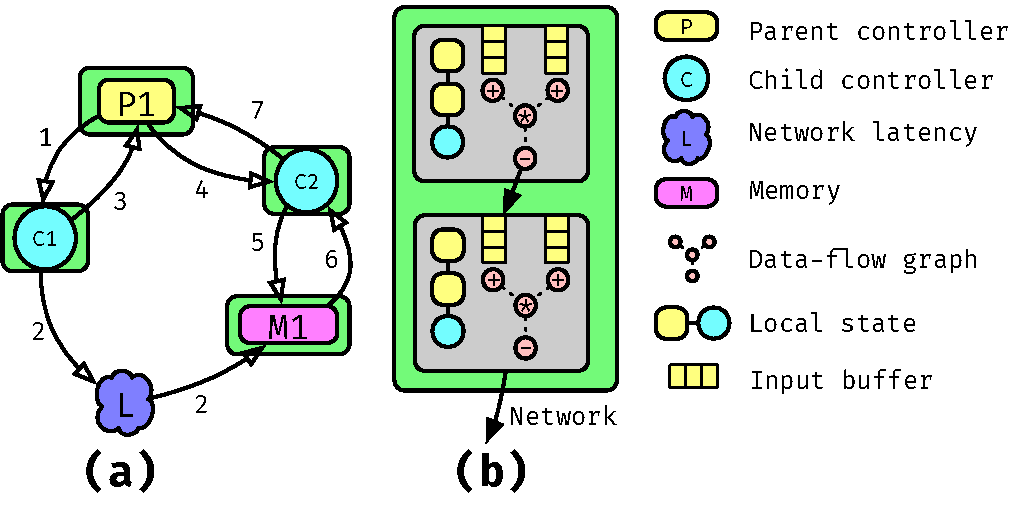
\includegraphics[height=0.12\paperheight]{figures/memory_inconsistency_actor_execution.pdf}
\caption{(a) Example of inconsistency in memory on a network with variable latency delay. (b) An actor that can execute data-flow graph of a leaf controller.}\label{fig:centralctrl} 
\label{fig:actor}
\end{figure}

\subsection{Input Control- and Data-Flow Graph}
\label{ssec:igraph}

The input to \name is a hierarchical control- and dataflow graph that captures the computation, memory, and control structure of the program. 
The control hierarchy (\Cref{fig:controller}, left) comprises of control constructs, such as loops and branches.
Each \emph{inner most} controller contains a data-flow graph (\Cref{fig:controller}, right) belonging to a basic block with a single control entrance and exit.
The input graph records intermediate memory accessed across controllers, carrying intermediate results of computations.
The control hierarchy encodes how many times the computation is repeated as well as in which order the intermediate memories are accessed.
A user or a high-level compiler determines which type and on/off-chip memory (such as DRAM, SRAM, or FIFO) the intermediate data reside in.

For on-chip SRAM, a user or a high-level compiler can \emph{statically partition} the memory and input to \name.
Static memory partitioning (or static banking)~\cite{poly_cong}, is a technique that statically transforms the data layout across memory partitions according 
to its access patterns in the program, such that parallel accesses do not have conflicts (accessing the same partition) at runtime.
A user can explicitly specify a bank ID and an offset to indicate which partition and address within the partition to access, like in CUDA~\cite{cuda}.
For a majority of access patterns, a high-level compiler\cite{spatial} can automatically solve and inject the address transformations into the program.
